\section{Technique and implementation}
%% \label{sec:approach}

\begin{figure*}
  \centering
  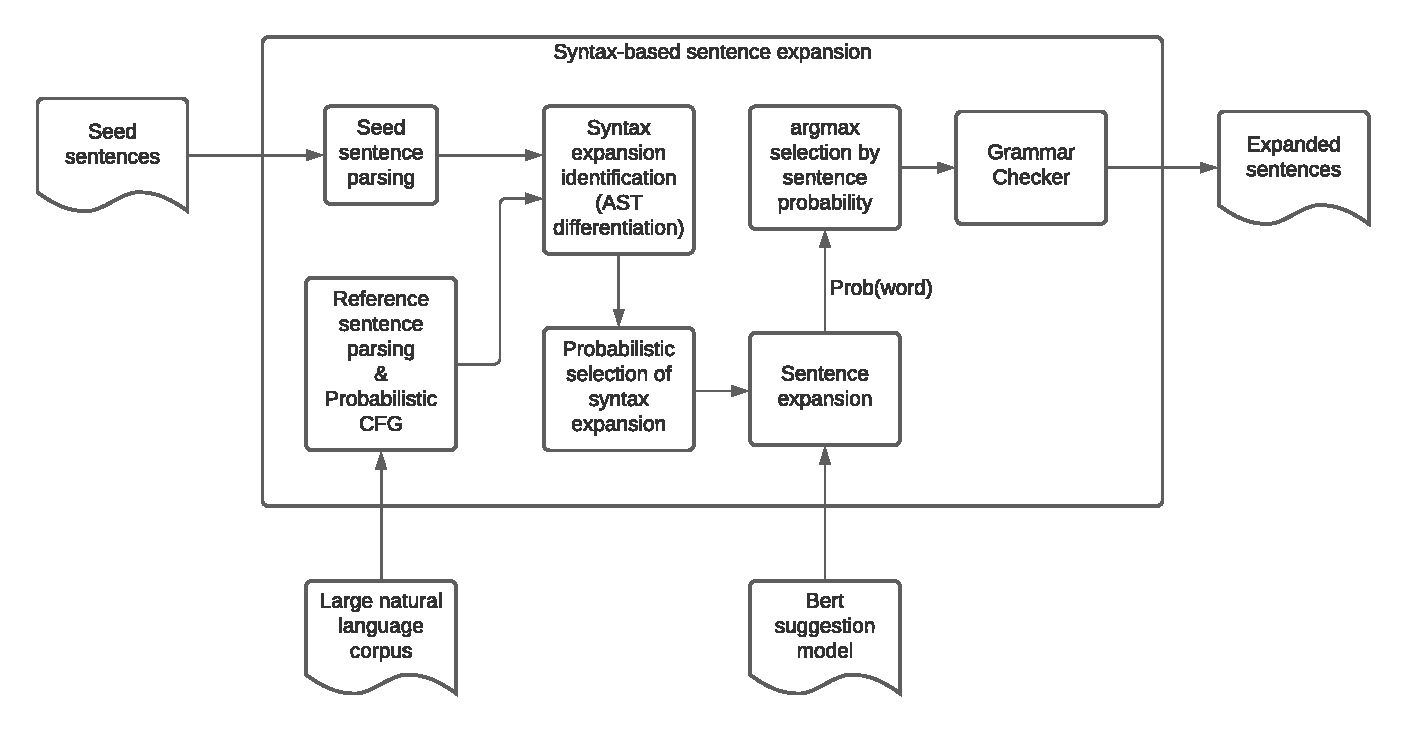
\includegraphics[scale=0.5]{figs/overall.pdf}
  \vspace{-5pt}
  \caption{\OverallModelFigCaption}
  \vspace{-10pt}
\end{figure*}

\Model generates input sentences with the following phases illustrated
in \ref{fig:OverallModel}: 1. search phase searches seed sentences according to
its requirement of \lc, 2. seed parsing phase parses the found seed
sentences and extract their \cfg, 3. reference phase collects large
corpus, 4. syntax expansion identification, and 5.sentence expansion
and generation. In this section, we provide more details on each phase.

\subsection{Search phase}
The search phase in \Model searches and samples subset of sentences in
the dataset that meets the requirement extracted from each linguistic
capability. The idea behind this phase 

In order to evaluate NLP models on \lc precisely, there
are two conditions in our interest.

First, inputs in the distrbution
characterized by each \lc is of importance. Each \lc represents
performance of NLP model on specific input distribution. Therefore,
the \lc introduces the constraints of the input distribution, and
input sentences from the constrained distribution are only qualified
to be used for evaluating the NLP model on the \lc.

In addition,
diversity in inputs is important to evaluate NLP models on the
\lc. The idea is that inputs that differ are more likely to cover the
NLP model behavior, and more coverage increases trustworthiness of the
evaluation. To achieve, we approach
